\chapter{ANÁLISE E DISCUSSÃO DE RESULTADOS}
\label{cap:resultados}
\renewcommand{\thetable}{\thechapter.\arabic{table}}
\renewcommand{\thefigure}{\thechapter.\arabic{figure}}
\setcounter{table}{0}\setcounter{figure}{0}
Este capítulo examina o desempenho das carteiras de Black-Litterman (BL) híbrido e de Markowitz em função do número de ativos, separando o efeito da alocação do efeito da seleção. A evidência principal corresponde ao experimento com cardinalidade n de 1 a 20, executado de 2 de janeiro a 30 de dezembro de 2025. A referência livre de risco é uma capitalização hipotética de 15\% ao ano, e 2024 é a janela anterior utilizada para escolher os horizontes quantitativos.

\section{Delimitação do experimento e critérios de comparação}
No cenário de ativos comuns, cada subconjunto permanece fixo no ano e é recebido pelos dois modelos, que atualizam os pesos mensalmente. No cenário de seleção própria, cada estratégia escolhe suas n ações a cada rebalanceamento. O primeiro desenho compara métodos de alocação sob as mesmas oportunidades; o segundo compara processos completos de seleção e alocação.

\begin{table}[H]
\centering
\caption{Condições da rodada consolidada.}
{\footnotesize
\begin{tabular}{p{0.40\linewidth}p{0.52\linewidth}}
\hline
Elemento & Condição \\ \hline
Capital inicial e período & R\$ 100.000; 250 observações em 2025 \\
Universo e cardinalidade & 20 ações; n = 1, 2, ..., 20 \\
Cenário comum & 551 subconjuntos; até 30 por n; semente fixa \\
Seleção própria & 20 trajetórias por modelo; seleção mensal \\
Total & 1.142 simulações individuais \\
Estimação e risco & Janela de 126 pregões; aversão ao risco = 3 \\
Posições e limites & Compra; piso 0,1\%; teto max(34,1677\%; 1/n) \\
Execução e custos & Fechamento seguinte ao sinal; 10 bps de turnover \\
Prior e notícias & Equilíbrio equiponderado; gate de 3 manchetes \\
\hline
\end{tabular}}
\par\smallskip{\footnotesize Fonte: elaboração própria, a partir do manifesto da simulação.}
\end{table}
São utilizadas todas as 20 combinações possíveis em n = 1 e n = 19 e o único conjunto em n = 20. Entre n = 2 e n = 18, avaliam-se 30 subconjuntos distintos por tamanho, sem enumeração exaustiva. As medianas e os percentis descrevem a dispersão entre conjuntos; não são intervalos de confiança nem a trajetória de uma carteira específica.

\noindent{\footnotesize O gate de três notícias foi adotado após comparar os limiares de 1 a 5 em 2025. Esta rodada é exploratória, não um teste independente do limiar. Os snapshots antigos não são agregados a estes resultados; a validade é discutida na Seção 4.7.}

\clearpage
\section{Desempenho quantitativo e escolha dos horizontes}
Os arquivos de previsões foram produzidos pelo procedimento walk-forward e reutilizados nesta avaliação. O horizonte de cada ativo foi escolhido pela acurácia direcional na validação de 2024, aceitando apenas alvos integralmente conhecidos antes de 2025. A Tabela 4.2 confronta essa medida com o diagnóstico de 2025, limitado a previsões cujo desfecho termina até 30 de dezembro. O número de pares é 245, 240 ou 229 para horizontes de 5, 10 ou 21 pregões, respectivamente.

\begin{table}[H]
\centering
\caption{Desempenho das previsões utilizadas no experimento.}
{\footnotesize
\begin{tabular}{@{}rrrrrr@{}}
\hline
Ativo & h & HR val. (\%) & HR 2025 (\%) & Maior classe (\%) & R$^{2}$ 2025 \\ \hline
ABEV3 & 5 & 57,72 & 45,71 & 49,80 & -0,098 \\
B3SA3 & 21 & 60,87 & 53,28 & 62,88 & -0,150 \\
BBAS3 & 10 & 64,61 & 43,75 & 50,42 & -0,138 \\
BBDC4 & 5 & 57,72 & 52,65 & 60,41 & -0,102 \\
CMIG4 & 21 & 71,30 & 61,14 & 65,94 & -0,357 \\
EQTL3 & 5 & 44,31 & 54,69 & 60,82 & -0,101 \\
GGBR4 & 21 & 68,70 & 44,10 & 61,57 & -0,301 \\
ITUB4 & 21 & 56,09 & 65,07 & 76,86 & -0,591 \\
LREN3 & 10 & 58,92 & 47,08 & 57,92 & -0,015 \\
MGLU3 & 21 & 68,70 & 47,60 & 52,40 & -0,440 \\
PETR3 & 10 & 68,88 & 46,67 & 52,92 & -0,115 \\
PETR4 & 21 & 62,61 & 54,59 & 51,53 & -0,099 \\
PRIO3 & 21 & 46,96 & 48,47 & 51,53 & -0,209 \\
RADL3 & 21 & 57,39 & 67,25 & 58,52 & -0,018 \\
RAIL3 & 21 & 52,61 & 55,46 & 55,02 & -0,011 \\
SANB11 & 21 & 63,98 & 56,33 & 64,19 & -0,189 \\
SBSP3 & 21 & 62,17 & 70,31 & 70,31 & -0,068 \\
SUZB3 & 10 & 47,72 & 37,08 & 62,92 & -0,111 \\
VALE3 & 10 & 64,04 & 33,75 & 71,25 & -0,335 \\
WEGE3 & 21 & 70,43 & 63,76 & 59,39 & 0,153 \\
\hline
\end{tabular}}
\par\smallskip{\footnotesize Fonte: elaboração própria. HR: acurácia direcional; h: pregões. A maior classe é uma referência descritiva ex post; não é uma regra de negociação escolhida previamente.}
\end{table}
A média simples da acurácia entre ativos cai de 60,29\% na validação para 52,44\% em 2025, redução de 7,85 pontos percentuais. O contraste evidencia que a seleção de um horizonte favorável em uma janela não assegura persistência no período seguinte. A avaliação financeira exige, portanto, análise própria, sem transformar a acurácia em expectativa direta de retorno.

\clearpage
\subsection*{Horizontes vencedores e alcance do sinal preditivo}
\begin{table}[H]
\centering
\caption{Distribuição dos horizontes e diagnóstico agregado.}
{\footnotesize
\begin{tabular}{p{0.40\linewidth}p{0.52\linewidth}}
\hline
Indicador & Resultado \\ \hline
Horizonte de 5 pregões & 3 ativos (15\%) \\
Horizonte de 10 pregões & 5 ativos (25\%) \\
Horizonte de 21 pregões & 12 ativos (60\%) \\
Mudanças frente ao vencedor do OOF completo & 4 dos 20 ativos \\
Acurácia média em 2025 & 52,44\% \\
R$^{2}$ negativo em 2025 & 19 dos 20 ativos \\
HR acima da classe majoritária & 4 ativos; 1 empate; 15 abaixo \\
\hline
\end{tabular}}
\par\smallskip{\footnotesize Fonte: elaboração própria, com base nas previsões por horizonte e nos preços locais.}
\end{table}
A predominância do horizonte de 21 pregões indica que a seleção temporal favoreceu sinais mais longos para a maior parte do universo, sem eliminar heterogeneidade entre empresas. A nova regra altera os horizontes de BBDC4, EQTL3, PETR3 e SUZB3 em relação aos arquivos de vencedores do OOF completo. Não se deve, assim, atribuir à rodada atual as métricas dos vencedores históricos sem verificar qual previsão foi efetivamente utilizada.

No conjunto completo dos vencedores históricos, a acurácia direcional média armazenada é 55,78\%, com R$^{2}$ negativo em 18 dos 20 ativos. Esses números pertencem a uma agregação mais ampla e a escolhas de estimador que podem consultar períodos posteriores a 2024. Por essa razão, funcionam como diagnóstico do treinamento, enquanto a Tabela 4.2 é a referência quantitativa desta discussão de 2025.

Os extremos do teste são SBSP3, com 70,31\% de acerto direcional, e VALE3, com 33,75\%. Entretanto, SBSP3 apenas empata com a frequência da classe majoritária, também de 70,31\%. Acertar mais da metade das observações não implica superar um referencial trivial de sinal. PETR4, RADL3, RAIL3 e WEGE3 superam essa referência descritiva; a maioria dos ativos permanece abaixo dela.

O R$^{2}$ avalia a magnitude prevista e pode ser negativo mesmo com acurácia direcional superior a 50\%. Em 2025, WEGE3 é a única exceção positiva, com R$^{2}$ de 0,153. O resultado dos demais ativos sugere erro quadrático superior ao da média retrospectiva da própria amostra avaliada, sem que essa média constitua uma previsão negociável. Como os alvos de vários pregões se sobrepõem, as observações não são independentes: não se interpreta a diferença para 50\% como significância estatística automática.

A conclusão quantitativa é de sinal heterogêneo e fraco na magnitude. Uma eventual vantagem da carteira precisa ser relacionada à combinação de prior, covariância, restrições e custos, e não tomada como prova isolada de qualidade do XGBoost.

\clearpage
\section{Comparação com ativos comuns}
A comparação pareada controla a composição elegível: os dois modelos recebem os mesmos papéis e operam nas mesmas datas. A diferença mediana é calculada primeiro dentro de cada par e depois agregada; ela pode diferir da subtração das duas medianas marginais. A Selic acumula 14,87\% nas 250 datas, em vez de 15\%, devido à convenção de 252 dias úteis por ano.

\begin{table}[H]
\centering
\caption{Retornos líquidos nos subconjuntos comuns.}
{\footnotesize
\begin{tabular}{@{}rrrrrr@{}}
\hline
n & Conjuntos & BL med. (\%) & MV med. (\%) & $\Delta$ pareado (p.p.) & BL > MV (\%) \\ \hline
1 & 20 & 21,26 & 21,26 & 0,00 & 0,0 \\
2 & 30 & 21,81 & 21,81 & 0,00 & 0,0 \\
3 & 30 & 32,88 & 32,06 & 0,47 & 70,0 \\
4 & 30 & 27,52 & 21,03 & 8,55 & 90,0 \\
5 & 30 & 27,85 & 19,33 & 11,13 & 83,3 \\
6 & 30 & 31,34 & 14,56 & 13,03 & 83,3 \\
7 & 30 & 32,58 & 14,28 & 17,01 & 96,7 \\
8 & 30 & 33,19 & 15,44 & 17,22 & 93,3 \\
9 & 30 & 31,90 & 13,32 & 20,95 & 93,3 \\
10 & 30 & 33,02 & 11,01 & 19,27 & 86,7 \\
11 & 30 & 28,61 & 6,05 & 23,52 & 100,0 \\
12 & 30 & 33,96 & 12,61 & 20,69 & 93,3 \\
13 & 30 & 32,60 & 11,77 & 18,91 & 96,7 \\
14 & 30 & 30,75 & 18,85 & 11,99 & 93,3 \\
15 & 30 & 31,48 & 20,89 & 9,62 & 80,0 \\
16 & 30 & 30,48 & 16,00 & 17,60 & 96,7 \\
17 & 30 & 30,38 & 19,39 & 11,31 & 93,3 \\
18 & 30 & 29,08 & 19,35 & 10,56 & 100,0 \\
19 & 20 & 28,59 & 19,25 & 9,28 & 95,0 \\
20 & 1 & 28,21 & 19,10 & 9,11 & 100,0 \\
\hline
\end{tabular}}
\par\smallskip{\footnotesize Fonte: elaboração própria. MV: Markowitz. A última coluna contabiliza vitórias estritas; os casos n = 1 e n = 2 têm 100\% de empates.}
\end{table}
A vantagem varia com a cardinalidade e a composição. Para n = 5, BL supera Markowitz em 83,3\% dos conjuntos, com diferença pareada mediana de 11,13 p.p. Para n = 10, a frequência é 86,7\% e a diferença mediana é 19,27 p.p. Essas frequências descrevem os subconjuntos avaliados, não probabilidades de vitória em outro ano.

\clearpage
\subsection*{Dispersão entre conjuntos e risco das carteiras}
\begin{figure}[H]
\centering
\caption{Retorno por cardinalidade com controle dos ativos elegíveis.}
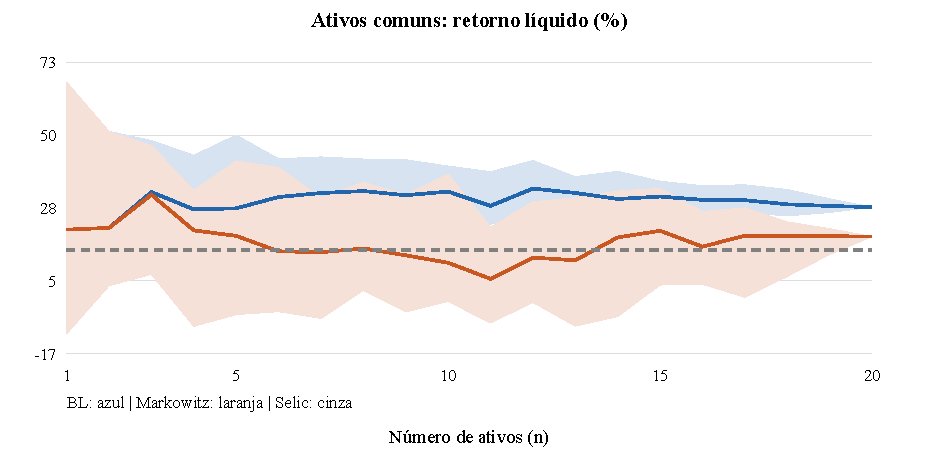
\includegraphics[width=\textwidth]{figuras/ativos_comuns.pdf}
\par\smallskip{\footnotesize Fonte: elaboração própria. Faixas: percentis entre subconjuntos, sem interpretação de intervalo de confiança.}
\end{figure}
\begin{table}[H]
\centering
\caption{Risco e desempenho ajustado nos conjuntos comuns.}
{\footnotesize
\begin{tabular}{@{}rrrrr@{}}
\hline
n & Modelo & Sharpe med. & Vol. anual (\%) & MDD med. (\%) \\ \hline
1 & BL & 0,34 & 26,85 & -21,47 \\
1 & Markowitz & 0,34 & 26,85 & -21,47 \\
5 & BL & 0,67 & 18,66 & -9,62 \\
5 & Markowitz & 0,31 & 19,10 & -12,94 \\
10 & BL & 0,89 & 17,35 & -8,44 \\
10 & Markowitz & -0,05 & 19,40 & -18,19 \\
20 & BL & 0,73 & 17,26 & -8,46 \\
20 & Markowitz & 0,29 & 19,23 & -12,78 \\
\hline
\end{tabular}}
\par\smallskip{\footnotesize Fonte: elaboração própria. Cada coluna é uma mediana marginal; não representa necessariamente o mesmo subconjunto.}
\end{table}
Para BL, os percentis de retorno em n = 5 são 12,88\% e 50,48\%; em n = 15, são 26,42\% e 36,25\%. A amplitude entre esses valores descreve a dependência da composição sorteada. Sua comparação permite avaliar robustez dentro do universo, sem assegurar generalização temporal.

Em n = 1, os métodos coincidem por investirem integralmente na mesma ação. Em n = 2, o teto de 50\% impõe pesos-alvo iguais. Para n = 3, o teto de 34,17\% deixa pouca liberdade de alocação. Portanto, as diferenças nos primeiros pontos também refletem restrições geométricas, e não apenas qualidade das estimativas.

\clearpage
\section{Comparação com seleção própria dos ativos}
Na escolha livre, cada modelo ranqueia os ativos pelo retorno esperado excedente dividido pela volatilidade histórica. Markowitz utiliza a média móvel; BL utiliza o posterior. A regra é explicitamente acrescentada à alocação: não corresponde à solução exaustiva do problema combinatório de selecionar a melhor carteira com n ações. Os retornos abaixo incluem seleção e distribuição de pesos.

\begin{table}[H]
\centering
\caption{Desempenho das estratégias com seleção própria.}
{\footnotesize
\begin{tabular}{@{}rrrrrrr@{}}
\hline
n & Ret. BL (\%) & Ret. MV (\%) & Sharpe BL & Sharpe MV & MDD BL (\%) & MDD MV (\%) \\ \hline
1 & -10,37 & 44,24 & -0,61 & 1,15 & -45,00 & -14,18 \\
2 & 66,12 & 32,41 & 1,32 & 0,83 & -24,91 & -11,16 \\
3 & 60,76 & 33,25 & 1,32 & 0,87 & -17,16 & -9,95 \\
4 & 62,72 & 23,33 & 1,60 & 0,46 & -12,62 & -11,94 \\
5 & 58,40 & 22,25 & 1,60 & 0,42 & -10,73 & -11,95 \\
6 & 49,34 & 20,07 & 1,34 & 0,33 & -10,68 & -12,68 \\
7 & 53,58 & 19,12 & 1,51 & 0,29 & -9,83 & -13,00 \\
8 & 45,86 & 18,78 & 1,30 & 0,27 & -8,20 & -13,00 \\
9 & 48,50 & 18,78 & 1,42 & 0,27 & -9,09 & -12,99 \\
10 & 40,14 & 18,84 & 1,13 & 0,27 & -10,20 & -12,97 \\
11 & 30,72 & 18,90 & 0,79 & 0,28 & -9,38 & -12,96 \\
12 & 36,11 & 18,88 & 1,03 & 0,28 & -7,57 & -12,95 \\
13 & 41,23 & 18,91 & 1,25 & 0,28 & -6,70 & -12,91 \\
14 & 34,78 & 18,96 & 0,99 & 0,28 & -6,70 & -12,89 \\
15 & 36,21 & 19,03 & 1,04 & 0,28 & -7,02 & -12,84 \\
16 & 35,69 & 19,09 & 1,04 & 0,28 & -7,28 & -12,82 \\
17 & 34,46 & 19,06 & 0,99 & 0,28 & -7,41 & -12,82 \\
18 & 33,80 & 19,05 & 0,96 & 0,28 & -8,04 & -12,82 \\
19 & 30,13 & 19,06 & 0,81 & 0,28 & -8,59 & -12,80 \\
20 & 28,21 & 19,10 & 0,73 & 0,29 & -8,46 & -12,78 \\
\hline
\end{tabular}}
\par\smallskip{\footnotesize Fonte: elaboração própria. Selic no período: 14,87\%. Há uma trajetória dinâmica por modelo e cardinalidade.}
\end{table}
BL supera Markowitz em retorno para 19 das 20 cardinalidades. Com uma ação, seu retorno é -10,37\%, contra 44,24\% de Markowitz, e seu drawdown é -45,00\%. Nesse caso, a distribuição de pesos é trivial: toda diferença decorre das ações escolhidas e das operações. A concentração exige atenção própria, mesmo quando carteiras maiores apresentam resultados favoráveis.

\clearpage
\subsection*{Trajetórias de capital e comparação com a renda fixa}
\begin{figure}[H]
\centering
\caption{Capital realizado em duas cardinalidades ilustrativas.}
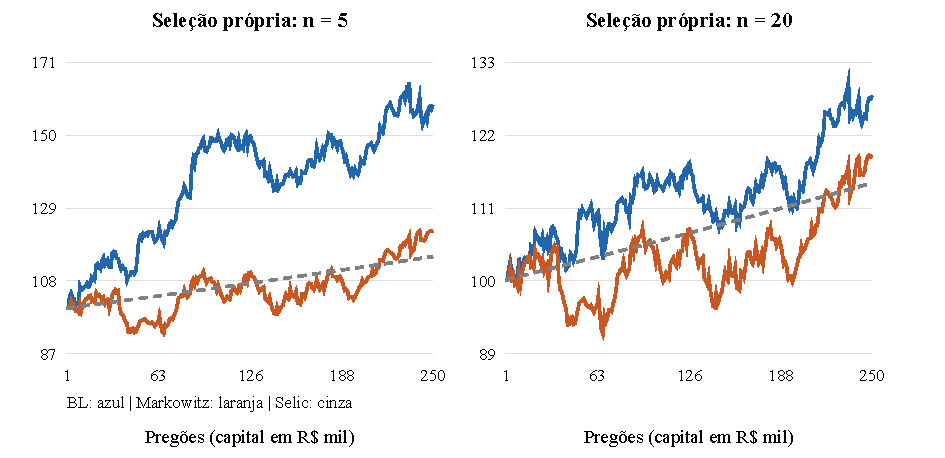
\includegraphics[width=\textwidth]{figuras/trajetorias_capital.pdf}
\par\smallskip{\footnotesize Fonte: elaboração própria. Capital inicial de R\$ 100 mil; custos de 10 bps. n = 5 é um exemplo, não uma seleção de tamanho feita antes do teste.}
\end{figure}
\begin{table}[H]
\centering
\caption{Resultado com todo o universo de vinte ativos.}
{\footnotesize
\begin{tabular}{@{}rrrr@{}}
\hline
Indicador & BL & Markowitz & Selic \\ \hline
Capital final (R\$) & 128.208,52 & 119.098,15 & 114.872,51 \\
Retorno líquido (\%) & 28,21 & 19,10 & 14,87 \\
Volatilidade anual (\%) & 17,26 & 19,23 & 0,00 \\
Sharpe sobre a Selic & 0,73 & 0,29 & Não definido \\
Drawdown máximo (\%) & -8,46 & -12,78 & 0,00 \\
\hline
\end{tabular}}
\par\smallskip{\footnotesize Fonte: elaboração própria. A Selic é uma série determinística; seu Sharpe não é definido por ter excesso e volatilidade nulos.}
\end{table}
Em n = 20, os cenários coincidem, pois todos os ativos são elegíveis. A diferença de retorno BL menos Markowitz é 9,11 p.p.; frente à Selic, é 13,34 p.p. As volatilidades são 17,26\% e 19,23\%, respectivamente. Essa comparação deve considerar também os drawdowns, pois a renda fixa não apresenta as oscilações das ações neste modelo simplificado.

O maior retorno de BL na escolha livre ocorre em n = 2, com 66,12\%; seu maior Sharpe ocorre em n = 4, com 1,60. Esses máximos foram identificados retrospectivamente, não validam um tamanho ótimo antes do teste. A capitalização estimada dos antigos CSVs não é comparada a estas curvas, pois pertence a outro motor e não constitui previsão compatível com este experimento.

\clearpage
\section{Sensibilidade à cardinalidade e aos custos de transação}
Na escolha livre de BL, os retornos em n = 1, n = 2 e n = 20 são, respectivamente, -10,37\%, 66,12\% e 28,21\%. A volatilidade passa de 32,48\% para 17,26\% entre os extremos. Não se presume melhora monotônica: aumentar n modifica as ações selecionadas, o risco de concentração e a liberdade de otimização.

\begin{table}[H]
\centering
\caption{Efeito dos custos nas estratégias com seleção própria.}
{\footnotesize
\begin{tabular}{@{}rrrrrr@{}}
\hline
n & Modelo & Sem custo (\%) & Líquido (\%) & Impacto (p.p.) & Custo pago (R\$) \\ \hline
1 & BL & -9,74 & -10,37 & 0,63 & 709,63 \\
1 & Markowitz & 45,25 & 44,24 & 1,01 & 735,18 \\
2 & BL & 67,56 & 66,12 & 1,44 & 1.176,03 \\
2 & Markowitz & 33,27 & 32,41 & 0,87 & 686,56 \\
5 & BL & 59,45 & 58,40 & 1,05 & 892,46 \\
5 & Markowitz & 23,01 & 22,25 & 0,76 & 639,14 \\
10 & BL & 40,91 & 40,14 & 0,78 & 681,41 \\
10 & Markowitz & 19,60 & 18,84 & 0,76 & 647,94 \\
20 & BL & 28,73 & 28,21 & 0,52 & 447,61 \\
20 & Markowitz & 19,85 & 19,10 & 0,75 & 644,25 \\
\hline
\end{tabular}}
\par\smallskip{\footnotesize Fonte: elaboração própria. O contrafactual sem custo mantém os mesmos pesos e operações, removendo apenas o desconto financeiro; não há nova otimização.}
\end{table}
O custo nominal pago e a perda de capital final não são a mesma medida: uma despesa antecipada também reduz o capital sujeito a retornos posteriores. Para n = 20, BL paga R\$ 447,61, com impacto de 0,52 p.p. de retorno. Markowitz paga R\$ 644,25, com impacto de 0,75 p.p.; seu turnover é 6,30, contra 4,05 de BL.

Em n = 2, BL tem turnover de 8,63 e custo de R\$ 1.176,03, com impacto de 1,44 p.p. Embora os pesos-alvo sejam 50/50, a troca das ações escolhidas e a restauração das proporções geram negociação. A comparação entre retorno bruto e líquido permite distinguir desempenho financeiro e despesas de implementação.

A rodada atual fixa a frequência mensal. Os antigos resultados diários e semanais e os experimentos de remoção de ativos utilizam outro motor e não são incorporados como sensibilidade diretamente comparável. A dispersão entre subconjuntos é uma análise de composição, mas não equivale a uma exclusão controlada de um ativo específico. Essas verificações exigem nova execução homogênea antes de receberem conclusões numéricas.

\clearpage
\section{Cobertura de notícias e influência efetiva das views}
O experimento utiliza gate de três notícias: a presença de pelo menos três manchetes no dia elegível habilita a view híbrida. Abaixo desse limiar, o hard prior reduz sua confiança a um valor próximo de zero. Para avaliar a influência potencial das views, a auditoria deve incidir sobre as datas mensais de decisão, e não apenas sobre a cobertura diária do ano.

\begin{table}[H]
\centering
\caption{Cobertura nas datas de formação dos sinais mensais.}
{\footnotesize
\begin{tabular}{@{}rrr@{}}
\hline
Indicador & Quantidade & Percentual \\ \hline
Pares ativo-data avaliados & 240 & 100,00\% \\
Com alguma notícia no dia elegível & 40 & 16,67\% \\
Com ao menos três notícias (gate = 3) & 6 & 2,50\% \\
Abaixo do gate & 234 & 97,50\% \\
Datas mensais com alguma view elegível & 3 de 12 & 25,00\% \\
\hline
\end{tabular}}
\par\smallskip{\footnotesize Fonte: elaboração própria, com base na auditoria de sinais. Notícias elegíveis: dia civil anterior ao sinal; universo de 20 ativos.}
\end{table}
O gate habilita 6 dos 240 pares ativo-data, presentes em 3 das doze datas mensais. Nas demais decisões, nenhuma ação atinge o mínimo de três manchetes. Esses números expressam cobertura informacional, não o tamanho exato da contribuição das views aos pesos. A regra é mais restritiva que a mera presença de uma notícia, embora quarenta pares contenham alguma manchete.

Nos ativos sem notícias elegíveis, a atualização permanece próxima do prior; nos demais, a mistura quantitativa e textual participa conforme a confiança estimada. A influência de uma opinião pode alcançar outros papéis pela estrutura de covariância. Por isso, o percentual de pares habilitados não deve ser interpretado diretamente como percentual da rentabilidade explicado pelas views.

A consulta apenas ao dia civil anterior ao sinal e a frequência mensal também limitam a informação utilizada: notícias em outros dias não geram rebalanceamento adicional. O gate de três foi adotado após a sensibilidade de 1 a 5 no próprio ano de 2025. Assim, o resultado descreve uma escolha retrospectiva, sem constituir validação independente do limiar nem evidência de irrelevância do sinal textual.

Não se compararam BL sem views, BL apenas quantitativo, BL apenas textual e híbrido completo sob um protocolo independente. Essa ablação continua necessária para atribuir ganhos a cada componente. A comparação atual identifica o desempenho do processo combinado frente a Markowitz e à Selic, mas não isola causalmente o valor incremental do XGBoost ou do sentimento.

\clearpage
\section{Limitações e alcance das conclusões}
A primeira limitação é temporal. Os horizontes foram escolhidos em 2024, mas a seleção original entre classificador e regressor pode ter consultado todo o OOF. Não houve retreinamento com seleção aninhada anterior ao teste. Além disso, o gate de três foi escolhido após observar o desempenho de 2025. A causalidade corrigida no motor não elimina esses problemas de seleção. A rodada é exploratória, não uma comprovação definitiva fora da amostra.

A segunda limitação é estatística. Há apenas um ano de avaliação financeira e vários tamanhos de carteira examinados. Os subconjuntos compartilham ações, datas e choques de mercado, de modo que 1.142 simulações não representam 1.142 amostras independentes. As frequências de vitória são descritivas. A escolha do melhor n pelo retorno de 2025 favoreceria uma configuração ex post; sua utilidade operacional exige validação anterior e teste em outro período, além de procedimentos que respeitem a dependência temporal.

A terceira limitação é de atribuição. Com gate de três notícias, 6 dos 240 pares ativo-data habilitam as views. A comparação não separa os efeitos do prior, das restrições, da covariância e das fontes de inteligência computacional. O diagnóstico quantitativo, com R$^{2}$ negativo em 19 ativos e acurácia inferior à classe majoritária em 15, reforça a necessidade de evitar inferências causais apenas pelo retorno agregado.

A quarta limitação é operacional. O universo é fixo, está sujeito a viés de sobrevivência e inclui classes de ações da mesma empresa, como PETR3 e PETR4; vinte papéis não equivalem a vinte fontes independentes de risco. A execução ao fechamento seguinte é uma aproximação, os custos são lineares e não se simulam spread, impacto de mercado, tributação ou liquidação terminal. O piso de 0,1\% mantém exatamente n posições, mas algumas podem ser economicamente pequenas.

Por fim, o prior neutro evita usar capitalização observada posteriormente, mas se afasta da especificação de equilíbrio ponderado por valor de mercado apresentada na arquitetura. A escala diária das views também é aproximada. O referencial de 15\% ao ano é uma taxa constante hipotética, e não a trajetória histórica da Selic. Essas convenções delimitam a comparação e precisam permanecer explícitas no procedimento experimental.

No universo completo, BL retorna 28,21\%, frente aos 19,10\% de Markowitz e aos 14,87\% da Selic. A vantagem nesta rodada com gate de três não demonstra superioridade geral: o limiar foi escolhido com conhecimento de 2025. A escolha de n e a contribuição de cada fonte também exigem validação independente.

